\chapter{Graphics}\label{cha:graphics}


\section{Meshes}\label{sec:Meshes}

Use the serial code \texttt{combine\_AVS\_DX.f90} (type `\texttt{make
combine\_AVS\_DX}' and then `\texttt{xcombine\_AVS\_DX}') to generate
AVS \urlwithparentheses{http://www.avs.com} output files (in AVS UCD format) or OpenDX \urlwithparentheses{http://www.opendx.org}
output files showing the mesh, the MPI partition (slices), the $\nchunks$
chunks, the source and receiver location, etc. Use the AVS UCD files
\texttt{AVS\_continent\_boundaries.inp} and \texttt{AVS\_plate\_boundaries.inp}
or the OpenDX files \texttt{DX\_continent\_boundaries.dx} and \texttt{DX\_plate\_boundaries.dx}
(that can be created using Perl scripts located in \texttt{UTILS/Visualization/opendx\_AVS})
for reference.


\section{Movies}\label{sec:Movies}

To make a surface or volume movie of the simulation, set parameters
\texttt{MOVIE\_SURFACE}, \texttt{MOVIE\_VOLUME}, and \texttt{NTSTEP\_BETWEEN\_FRAMES}
in the \texttt{Par\_file}. Turning on the movie flags, in particular
\texttt{MOVIE\_VOLUME}, produces large output files. \texttt{MOVIE\_VOLUME}
files are saved in the \texttt{LOCAL\_PATH} directory, whereas \texttt{MOVIE\_SURFACE}
output files are saved in the \texttt{OUTPUT\_FILES} directory. We
save the velocity field. The look of a movie is determined by the
half-duration of the source. The half-duration should be large enough
so that the movie does not contain frequencies that are not resolved
by the mesh, i.e., it should not contain numerical noise. This can
be accomplished by selecting a CMT \texttt{HALF\_DURATION} > 1.1 $\times$
smallest period (see figure \ref{fig:CMTSOLUTION-file}). When \texttt{\small MOVIE\_SURFACE}
= \texttt{\small .true.} or \texttt{\small MOVIE\_VOLUME}{\small{}
}\texttt{\small =}{\small{} }\texttt{\small .true.}, the half duration
of each source in the \texttt{CMTSOLUTION} file is replaced by

\begin{quote}
\[
\sqrt{(}\mathrm{\mathtt{HALF\_DURATIO}\mathtt{N}^{2}}+\mathrm{\mathtt{HDUR\_MOVI}\mathtt{E}^{2}})\]
\textbf{NOTE:} If \texttt{HDUR\_MOVIE} is set to 0.0, the code will
select the appropriate value of 1.1 $\times$ smallest period. As
usual, for a point source one can set \texttt{HALF\_DURATION} in the
\texttt{Par\_file} to be 0.0 and \texttt{HDUR\_MOVIE} = 0.0 to get
the highest frequencies resolved by the simulation, but for a finite
source one would keep all the \texttt{HALF\_DURATION}s as prescribed
by the finite source model and set \texttt{HDUR\_MOVIE} = 0.0.
\end{quote}

\subsection{Movie Surface}

When running \texttt{xspecfem3D} with the \texttt{MOVIE\_SURFACE}
flag turned on the code outputs \texttt{moviedata??????} files in
the \texttt{OUTPUT\_FILES} directory. The files are in a fairly complicated
binary format, but there are two programs provided to convert the
output into more user friendly formats. The first one, \texttt{create\_movie\_AVS\_DX.f90}
outputs data in ASCII, OpenDX, AVS, or ParaView format. Run the code
from the source directory (type `\texttt{make} \texttt{create\_movie\_AVS\_DX}'
first) to create an input file in your format of choice. The code
will prompt the user for input parameters. The second program \texttt{create\_movie\_GMT\_global.f90}
outputs ASCII xyz files, convenient for use with GMT. This codes uses
significantly less memory than \texttt{create\_movie\_AVS\_DX.f90}
and is therefore useful for high resolution runs.
A README file and sample Perl scripts to create movies using GMT are provided in directory
\texttt{UTILS/Visualization/GMT}.

%
\begin{figure}[H]
\noindent \begin{centering}
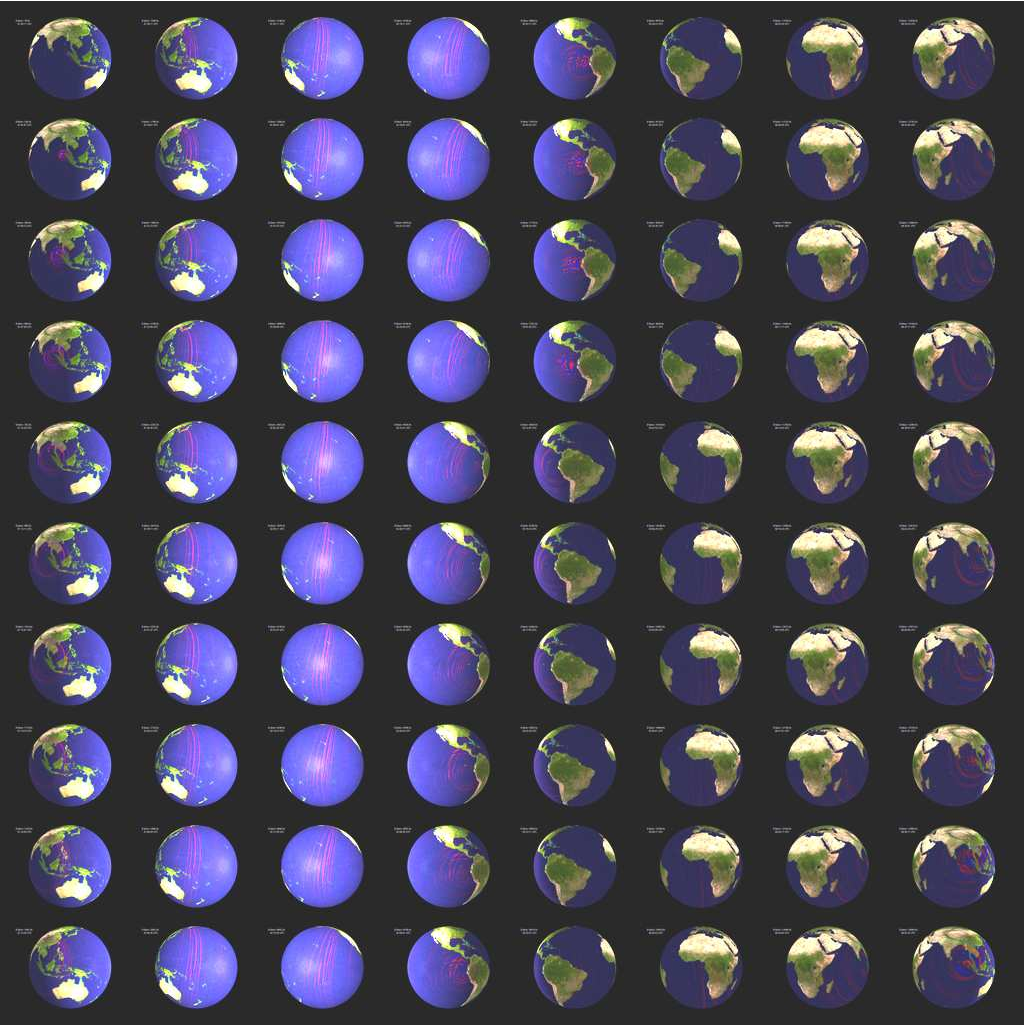
\includegraphics[scale=0.75]{figures/geo-poster4_small.pdf}
\par\end{centering}

\caption{Snapshots from a global movie for the December 26, 2004, M=9.2 Sumatra-Andaman
earthquake. Time runs down successive columns.}

\end{figure}



\subsection{Movie Volume}\label{sub:Movie-Volume}

When running xspecfem3D with the \texttt{\small MOVIE\_VOLUME} flag
turned on, the code outputs several files in \texttt{\small LOCAL\_DIR}.
As the files can be very large, there are several flags in the \texttt{\small Par\_file}
that control the region in space and time that is saved. These are:
\texttt{\small MOVIE\_TOP\_KM}, \texttt{\small MOVIE\_BOTTOM\_KM},
\texttt{\small MOVIE\_WEST\_DEG}, \texttt{\small MOVIE\_EAST\_DEG},
\texttt{\small MOVIE\_NORTH\_DEG}, \texttt{\small MOVIE\_SOUTH\_DEG},
\texttt{\small MOVIE\_START} and \texttt{\small MOVIE\_STOP}. The
code will save a given element if the center of the element is in
the prescribed volume.

\begin{description}
\item [{The~Top/Bottom:}] Depth below the surface in kilometers, use \texttt{\small MOVIE\_TOP}
\texttt{\small =} \texttt{\small -100.0} to make sure the surface
is stored.
\item [{West/East:}] Longitude, degrees East {[}-180.0/180.0]
\item [{North/South:}] Latitute, degrees North {[}-90.0/90.0]
\item [{Start/Stop:}] Frames will be stored at \texttt{\small MOVIE\_START}
\texttt{\small +} \texttt{\small i{*}NSTEP\_BETWEEN\_FRAMES}, where
\texttt{\small i=(0,1,2..)} while \texttt{\small i{*}NSTEP\_BETWEEN\_FRAMES}
\texttt{\small <=} \texttt{\small MOVIE\_STOP}{\small \par}
\end{description}
The code saves several files, and the output is saved by each processor.
The first is \texttt{\small proc??????\_movie3D\_info.txt} which contains
two numbers, first the number of points within the prescribed volume
within this particular slice, and second the number of elements. The
next files are \texttt{\small proc??????\_movie3D\_x.bin}, \texttt{\small proc??????\_movie3D\_y.bin},
\texttt{\small proc??????\_movie3D\_z.bin} which store the locations
of the points in the 3D mesh.

Finally the code stores the ``value'' at each of the points. Which
value is determined by \texttt{\small MOVIE\_VOLUME\_TYPE} in the
\texttt{\small Par\_file}. Choose 1 to save the strain, 2 to save
the time integral of strain, and 3 to save $\mu${*}time integral
of strain in the subvolume. Choosing 4 causes the code to save the
trace of the stress and the deviatoric stress in the whole volume
(not the subvolume in space), at the time steps specified. The name
of the output file will depend on the \texttt{\small MOVIE\_VOLUME\_TYPE}
chosen.

Setting \texttt{\small MOVIE\_VOLUME\_COARSE} \texttt{\small =} \texttt{\small .true.}
will make the code save only the corners of the elements, not all
the points within each element for \texttt{\small MOVIE\_VOLUME\_TYPE}
\texttt{\small =} \texttt{\small 1,2,3}.

To make the code output your favorite ``value'' simply add a new \texttt{\small MOVIE\_VOLUME\_TYPE},
a new subroutine to \texttt{\small write\_movie\_volume.f90} and a
subroutine call to \texttt{\small specfem3D.F90}.

A utility program to combine the files produced by \texttt{\small MOVIE\_VOLUME\_TYPE}
\texttt{\small =} \texttt{\small 1,2,3} is provided in \texttt{\small combine\_paraview}~\\
\texttt{\small \_strain\_data.f90}. Type \texttt{\small xcombine\_paraview\_strain\_data}
to get the usage statement. The program \texttt{\small combine\_vol}~\\
\texttt{\small \_data.f90} can be used for \texttt{\small MOVIE\_VOLUME\_TYPE}
\texttt{\small =} \texttt{\small 4}.


\section{Finite-Frequency Kernels}\label{sec:Finite-Frequency-Kernels}

The finite-frequency kernels computed as explained in Section \ref{sec:Adjoint-simulation-finite}
are saved in the \texttt{LOCAL\_PATH} at the end of the simulation.
Therefore, we first need to collect these files on the front end,
combine them into one mesh file, and visualize them with some auxilliary
programs. Examples of kernel simulations may be found in the \texttt{EXAMPLES} directory.

\begin{enumerate}
\item \textbf{Create slice files}


We will only discuss the case of one source-receiver pair, i.e., the
so-called banana-doughnut kernels. Although it is possible to collect
the kernel files from all slices onto the front end, it usually takes
up too much storage space (at least tens of gigabytes). Since the
sensitivity kernels are the strongest along the source-receiver great
circle path, it is sufficient to collect only the slices that are
along or close to the great circle path.

A Perl script \texttt{UTILS/Visualization/Paraview/global\_slice\_number.pl} can
help to figure out the slice numbers that lie along the great circle
path (both the minor and major arcs), as well as the slice numbers
required to produce a full picture of the inner core if your kernel
also illuminates the inner core.

\begin{enumerate}
\item You need to first compile the utility programs provided in the \texttt{UTILS/Visualization/Paraview/}~\\
\texttt{global\_slice\_util
}directory. Then copy the \texttt{CMTSOLUTION} file, \texttt{STATIONS\_ADJOINT},
and \texttt{Par\_file}, and run:

\begin{lyxcode}
global\_slice\_number.pl~CMTSOLUTION~STATIONS\_ADJOINT~Par\_file
\end{lyxcode}
In the case of visualization boundary kernels or spherical cross-sections
of the volumetric kernels, it is necessary to obtain the slice numbers
that cover a belt along the source and receiver great circle path,
and you can use the hybrid version:

\begin{lyxcode}
globe\_slice\_number2.pl~CMTSOLUTION~STATIONS\_ADJOINT~

~~~~~Par\_file~belt\_width\_in\_degrees
\end{lyxcode}
A typical value for \texttt{belt\_width\_in\_degrees} can be 20.

\item For a full 6-chunk simulation, this script will generate the \texttt{slice\_minor},
\texttt{slice\_major}, \texttt{slice\_ic} files, but for a one-chunk simulation, this script only generates the \texttt{slice\_minor}
file.
\item For cases with multiple sources and multiple receivers, you need to
provide a slice file before proceeding to the next step.
\end{enumerate}
\item \textbf{Collect the kernel files}


After obtaining the slice files, you can collect the corresponding
kernel files from the given slices.

\begin{enumerate}
\item To accomplish this, you can use or modify the scripts in \texttt{UTILS/collect\_database
}directory:

\begin{lyxcode}
{\small copy\_m(oc,ic)\_globe\_database.pl~slice\_file~lsf\_machine\_file~filename~{[}jobid]}{\small \par}
\end{lyxcode}
for volumetric kernels, where \texttt{\small lsf\_machine\_file} is
the machine file generated by the LSF scheduler, \texttt{\small filename}
is the kernel name (e.g., \texttt{\small rho\_kernel}, \texttt{\small alpha\_kernel}
and \texttt{\small beta\_kernel}), and the optional \texttt{\small jobid}
is the name of the subdirectory under \texttt{\small LOCAL\_PATH}
where all the kernel files are stored. For boundary kernels, you need
to use

\begin{lyxcode}
{\small copy\_surf\_globe\_database.pl~slice\_file~lsf\_machine\_file~filename~{[}jobid]}{\small \par}
\end{lyxcode}
where the filename can be \texttt{\small Moho\_kernel}, \texttt{\small d400\_kernel},
\texttt{\small d670\_kernel}, \texttt{\small CMB\_kernel} and \texttt{\small ICB\_kernel}.

\item After executing this script, all the necessary mesh topology files
as well as the kernel array files are collected to the local directory
on the front end.
\end{enumerate}
\item \textbf{Combine kernel files into one mesh file}


We use an auxiliary program \texttt{combine\_vol\_data.f90} to combine
the volumetric kernel files from all slices into one mesh file, and
\texttt{combine\_surf\_data.f90 }to combine the surface kernel files.

\begin{enumerate}
\item Compile it in the global code directory:

\begin{lyxcode}
{\footnotesize make~combine\_vol\_data~}{\footnotesize \par}

{\footnotesize ./bin/xcombine\_vol\_data}~{\footnotesize slice\_list}~{\footnotesize kernel\_filename}~
{\footnotesize input\_topo\_dir}~
{\footnotesize input\_file\_dir}~{\footnotesize output\_dir}

{\footnotesize low/high-resolution-flag-0-or-1}~{\footnotesize {[}region]}{\footnotesize \par}
\end{lyxcode}
where \texttt{input\_dir} is the directory where all the individual
kernel files are stored, and \texttt{output\_dir} is where the mesh
file will be written. Give 0 for low resolution and 1 for high resolution.
If region is not specified, all three regions (crust and mantle, outer core, inner core)
will be collected, otherwise, only the specified region will be.
Here is an example:
\texttt{./xcombine\_vol\_data slices\_major alpha\_kernel input\_topo\_dir}
\texttt{~~~~~~~~~~~~~~~~~~~~~~~~~~~~~input\_file\_dir output\_dir 1}

\begin{lyxcode}
{\footnotesize ./bin/xcombine\_surf\_data~slice\_list~filename~surfname~input\_dir~output\_dir}
{\footnotesize ~~~~~~~~~~~~~~~~~~~~~~~~~~~~~~~~~low/high-resolution~2D/3D}{\footnotesize \par}
\end{lyxcode}
where \texttt{surfname} should correspond to the specific kernel file
name, and can be chosen from \texttt{Moho}, \texttt{400}, \texttt{670},
\texttt{CMB} and \texttt{ICB}.

\item Use 1 for a high-resolution mesh, outputting all the GLL points to
the mesh file, or use 0 for low resolution, outputting only the corner
points of the elements to the mesh file. Use 0 for 2D surface kernel
files and 1 for 3D volumetric kernel files.
\item Use region = 1 for the mantle, region =2 for the outer core, region
= 3 for the inner core, and region = 0 for all regions.
\item The output mesh file will have the name \texttt{reg\_?\_rho(alpha,beta)\_kernel.mesh,}
or\texttt{ }~\\
\texttt{reg\_?\_Moho(d400,d670,CMB,ICB)\_kernel.surf.}
\end{enumerate}
\item \textbf{Convert mesh files into .vtu files}

\begin{enumerate}
\item We next convert the \texttt{.mesh} file into the VTU (Unstructured
grid file) format which can be viewed in ParaView, for example:

\begin{lyxcode}
mesh2vtu~-i~file.mesh~-o~file.vtu
\end{lyxcode}
\item Notice that this program \texttt{mesh2vtu}, in the
\texttt{UTILS/Visualization/Paraview/mesh2vtu} directory, uses the
VTK \urlwithparentheses{http://www.vtk.org} run-time library for its execution. Therefore,
make sure you have it properly installed.
\end{enumerate}
\item \textbf{Copy over the source and receiver .vtk file}


In the case of a single source and a single receiver, the simulation
also generates the \texttt{OUTPUT\_FILES/sr.vtk} file to describe
the source and receiver locations, which can be viewed in Paraview
in the next step.

\item \textbf{View the mesh in ParaView}


Finally, we can view the mesh in ParaView \urlwithparentheses{http://www.paraview.org}.

\begin{enumerate}
\item Open ParaView.
\item From the top menu, \textsf{File} $\rightarrow$\textsf{ Open data},
select \texttt{file.vtu}, and click the \textsf{Accept} button.

\begin{itemize}
\item If the mesh file is of moderate size, it shows up on the screen; otherwise,
only the outline is shown.
\end{itemize}
\item Click \textsf{Display Tab} $\rightarrow$ \textsf{Display Style} $\rightarrow$
\textsf{Representation} and select \textsf{wireframe of surface} to
display it.
\item To create a cross-section of the volumetric mesh, choose \textsf{Filter}
$\rightarrow$ \textsf{cut}, and under \textsf{Parameters Tab}, choose
\textsf{Cut Function} $\rightarrow$ \textsf{plane}.
\item Fill in center and normal information given by the standard output
from \texttt{global\_slice\_number.pl} script.
\item To change the color scale, go to \textsf{Display Tab} $\rightarrow$
\textsf{Color} $\rightarrow$ \textsf{Edit Color Map} and reselect
lower and upper limits, or change the color scheme.
\item Now load in the source and receiver location file by \textsf{File}
$\rightarrow$\textsf{ Open data}, select \texttt{sr.vt}k, and click
the \textsf{Accept} button. Choose \textsf{Filter} $\rightarrow$\textsf{
Glyph}, and represent the points by `\textsf{spheres}'.
\item For more information about ParaView, see the ParaView Users Guide \urlwithparentheses{http://www.paraview.org/files/v1.6/ParaViewUsersGuide.PDF}.
\end{enumerate}
\end{enumerate}
For illustration purposes, Figure \ref{fig:P-wave-speed-finite-frequency}
shows P-wave speed finite-frequency kernels from cross-correlation traveltime and amplitude measurements for a P arrival recorded at an epicentral distance of $60^{\circ}$ for a deep event.

%
\begin{figure}[H]
\noindent \begin{centering}
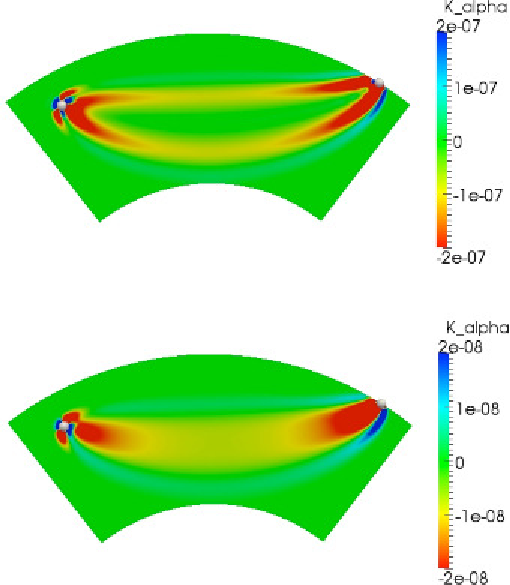
\includegraphics[clip,scale=1.2]{figures/P_alpha_60d_17s.pdf}
\caption{P-wave speed finite-frequency
kernels from cross-correlation traveltime (top) and amplitude (bottom) measurements
for a P arrival recorded at an epicentral distance of $60^{\circ}$.
The kernels together with the associated files and routines to reproduce them
may be found in \texttt{EXAMPLES/global\_PREM\_kernels/}.
}
\label{fig:P-wave-speed-finite-frequency}
\par\end{centering}
\end{figure}



